\documentclass[french]{beamer}

\usepackage[utf8]{inputenc}
\usepackage[T1]{fontenc}
\usepackage{lmodern}
\usepackage{amsmath, amssymb}
\usepackage{graphicx}
\usepackage{babel}
\usepackage{listings}

\usetheme{Warsaw}

\useinnertheme[shadow=true]{rounded}
\useoutertheme{shadow}
\usecolortheme{orchid}
\usecolortheme{whale}


\title{The GIMP : Traitement d'image}
\subtitle{Présentation de TCCP}
\author[Latour - Galand]{Latour Pierre-Louis - Galand Simon}
\date{Année 2014-2015}
\institute[UM2-FDS]{Université Montpellier 2 - Faculté des sciences}

\begin{document}
    \begin{frame}
	    \titlepage
	    \begin{center}
	    
\includegraphics[height=1.5cm]{logo.jpeg}
	    \end{center}
    \end{frame}

    \begin{frame}{Sommaire}
	    \small\tableofcontents
    \end{frame}
    
    
    \section{Les images}
        \begin{frame}{Les images}
            \tableofcontents[currentsection, hideallsubsections]
        \end{frame}
        
        \subsection{Définition}
            \begin{frame}{Définitions}
                \tableofcontents[sectionstyle=show/hide,subsectionstyle=show/shaded/hide]                             \end{frame}
                
            \begin{frame}
                \begin{center}
                    \begin{block}{Définition}
                        Une image est une représentation visuelle (ou mentale) de quelque chose. Elle peut  être "naturelle" ou "de synthèse". 
                    \end{block}
                \end{center}
            \end{frame}
            
            \begin{frame}{Types d'images}
                \begin{block}{Image Naturelle}
                        Une image naturelle est une vue d'objet réelle capturée par un système photographique.
                \end{block}
                \begin{block}{Image de Synthèse}
                        Une image de synthèse est une image conçu numériquement par l'application d'un modèle physique.
                \end{block}
            \end{frame}
            \begin{frame}
                \begin{exampleblock}{Exemple d'image Naturelle}
	               Photo:\\
	               \begin{center}
	                    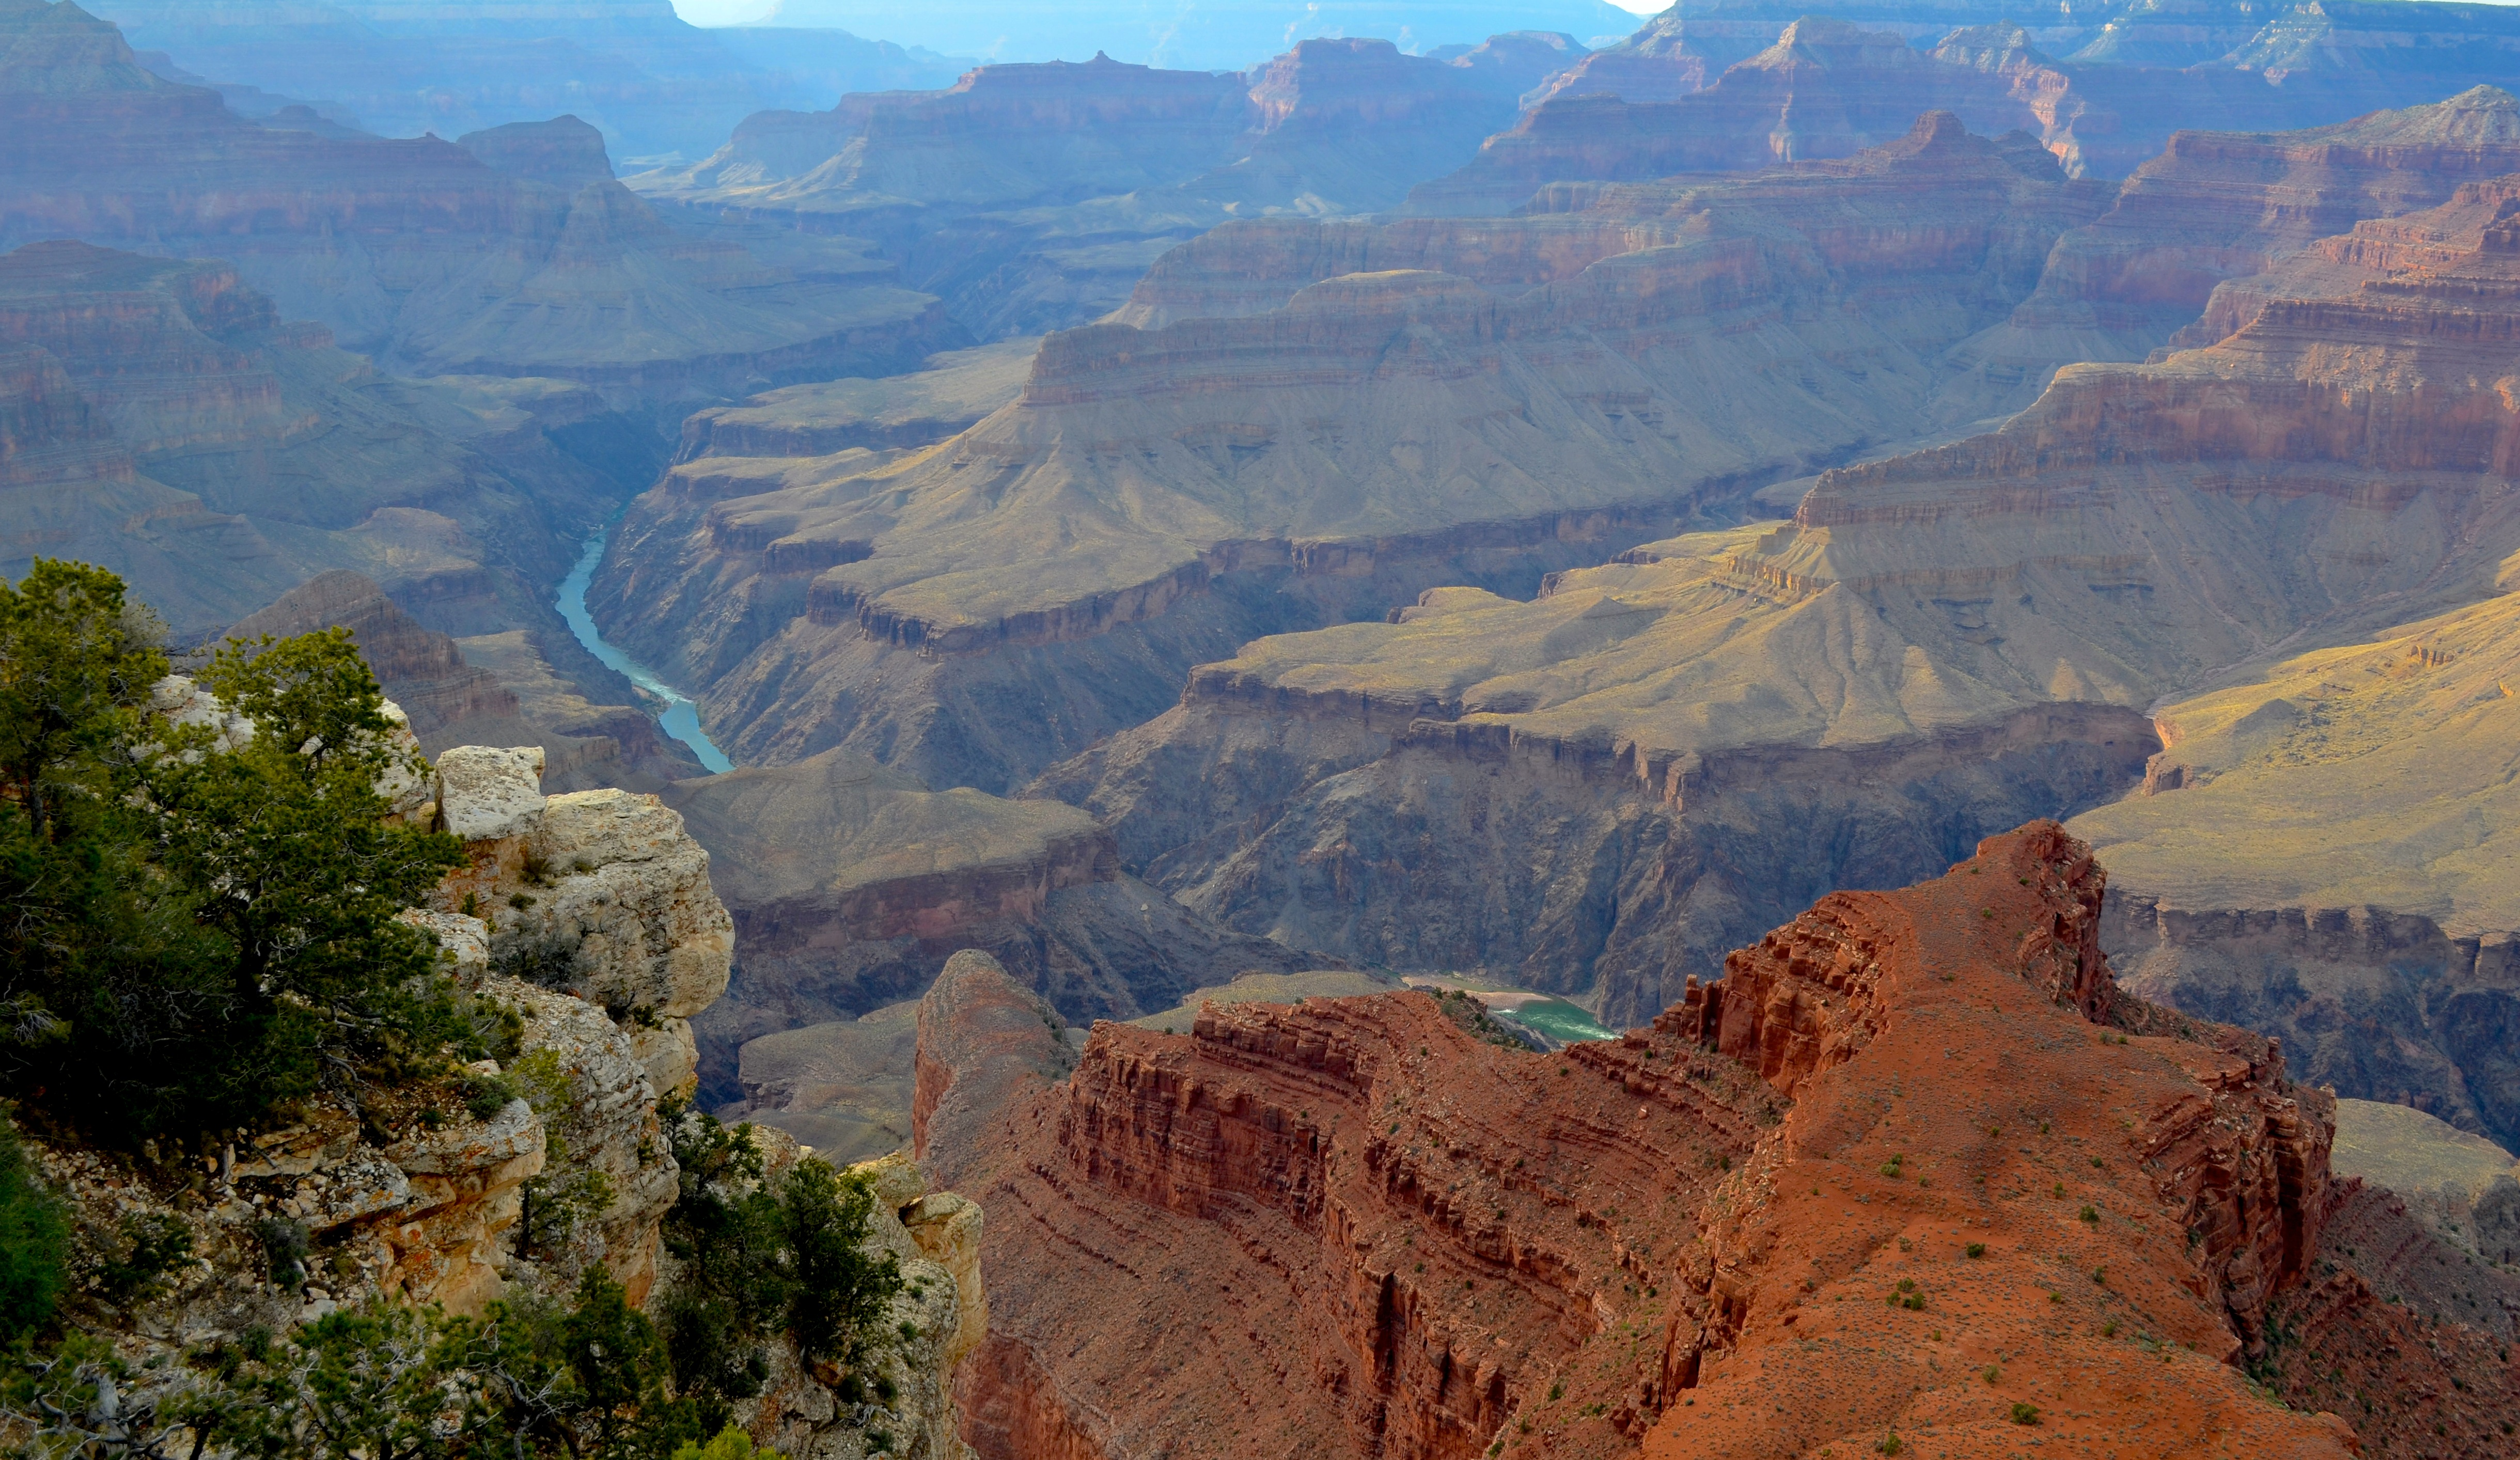
\includegraphics[width=3.7cm]{photo_naturelle.jpg}
	               \end{center}
            	\end{exampleblock}
            	\begin{exampleblock}{Exemple d'image de Synthèse}
                    Modélisation 3D:\\
                    \begin{center}
	                    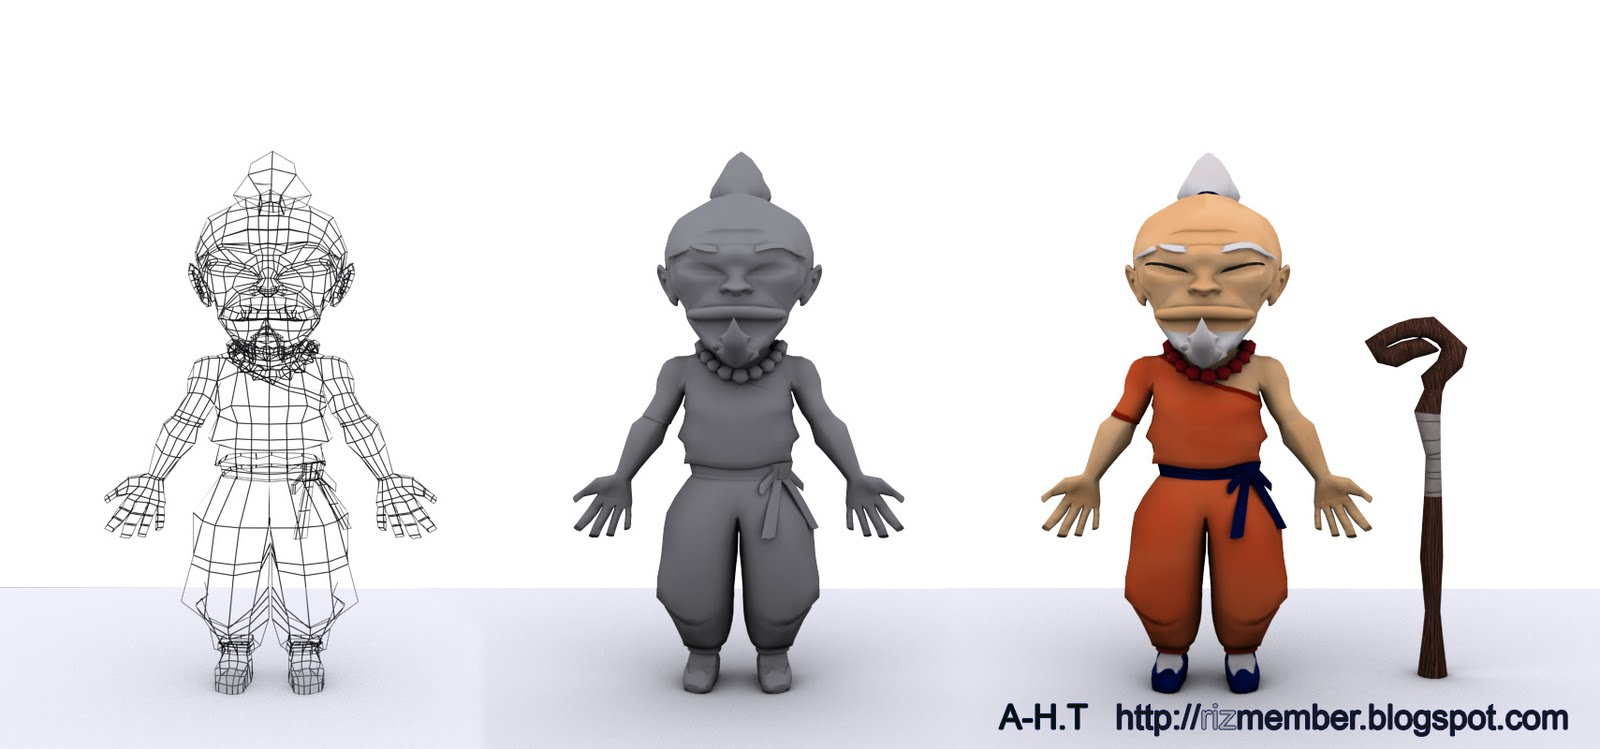
\includegraphics[width=4cm]{Image_synthese.jpg}
	                \end{center}
            	\end{exampleblock}
            \end{frame}
            
        \subsection{Images numériques}
            \begin{frame}{Images numériques}
                \tableofcontents[sectionstyle=show/hide,subsectionstyle=show/shaded/hide]
            \end{frame}
            \begin{frame}
                En Informatique, les images sont visualisables sous forme numérique.
                \begin{block}{Qu'est ce qu'une image numérique?}
                        Une image dite "numérique" désigne toute image (dessin, icône, photographie,...) acquise, créée, traitée, et stockée sous forme binaire.\\
                        Celle-ci peut être matricielle ou vectorielle.\\
                \end{block}
            \end{frame}
            \begin{frame}
                \begin{exampleblock}{Exemple d'image matricielle}
                    \begin{center}
                        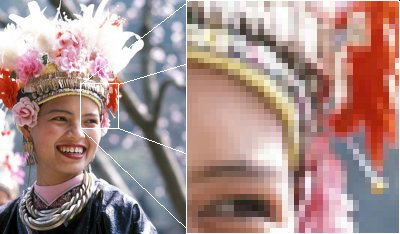
\includegraphics[width=3.5cm]{Image_matricielle.jpg}
	                \end{center}
            	\end{exampleblock}
            	\begin{exampleblock}{Exemple d'image vectorielle comparée à une image matricielle}
                    \begin{center}
	                    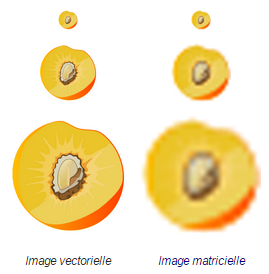
\includegraphics[width=3.4cm]{img_vectimg_matr.png}
	                \end{center}
            	\end{exampleblock}
            \end{frame}

            
    \section{Le traitement d'image}
        \begin{frame}{Le Traitement d'image}
            \tableofcontents[currentsection, hideallsubsections]
        \end{frame}
        
        \subsection{Définition}
            \begin{frame}{Définition}
                \tableofcontents[sectionstyle=show/hide,subsectionstyle=show/shaded/hide]
            \end{frame}
            \begin{frame}
                \begin{center}
                    \begin{block}{Définition}
                        Le traitement d'image est une discipline mêlant informatique et mathématiques appliquées, qui a pour but de modifier une image numérique ou d'en extraire des informations.
                    \end{block}
                \end{center}
            \end{frame}
        \subsection{Types de traitements}
            \begin{frame}{Types de traitements}
                \tableofcontents[sectionstyle=show/hide,subsectionstyle=show/shaded/hide]
            \end{frame}
            \begin{frame}
                De manière générale on divise le traitement d'image en deux parties distinctes:
                \begin{itemize}
                    \item La transformation: Transformer une image A en une image B par une modification du code de la première.
                    \item L'extraction: Extraire une information d'une image pour accomplir une tâche.
                \end{itemize}
            \end{frame}
            
        \subsection{Applications}
            \begin{frame}{Applications}
               \tableofcontents[sectionstyle=show/hide,subsectionstyle=show/shaded/hide]
            \end{frame}
            \begin{frame}
                On fait du traitement d'image lorsque:
                \begin{itemize}
                    \item On retouche une image
                    \item On cherche à vérifier la qualité d'un produit (exemple: colorimétrie)
                    \item On essaye d'identifier les ressemblances entre deux images (exemple: reconnaissance faciale, biométrique...)
                    \item Et bien d'autres applications existantes et possibles...
                \end{itemize}
            \end{frame}
            \begin{frame}
                \begin{exampleblock}{Exemple de retouche sur un magazine}
                    \begin{center}
	                    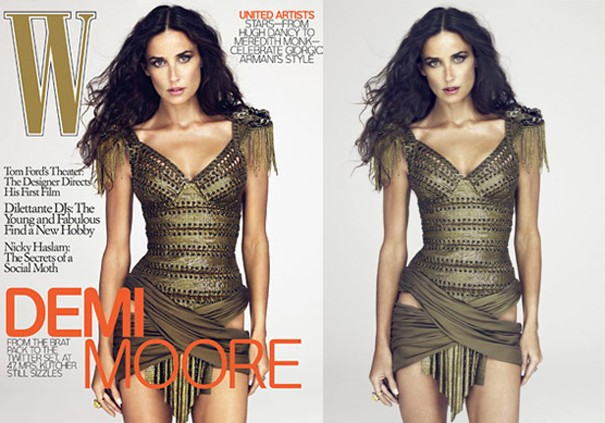
\includegraphics[width=5cm]{retouche_magazine.jpg}
	                \end{center}
            	\end{exampleblock}
            \end{frame}
        \subsection{Outils de traitement}
            \begin{frame}{Outils de traitement}
               \tableofcontents[sectionstyle=show/hide,subsectionstyle=show/shaded/hide]
            \end{frame}
            \begin{frame}
            Il existe différents outils de manipulation des images tels que:
                \begin{itemize}
                    \item Les opérateurs pixel à pixel (ou point à point)
                    \item Les opérateurs locaux
                    \item Les opérateurs dans l'espace fréquentiel
                \end{itemize}
                Ceci n'étant qu'une liste non-exhaustive.
            \end{frame}
    \section{The GIMP}
        \begin{frame}{The GIMP}
            \tableofcontents[currentsection, hideallsubsections]
        \end{frame}
        \subsection{Présentation}
            \begin{frame}{Présentation}
                \tableofcontents[sectionstyle=show/hide,subsectionstyle=show/shaded/hide]
            \end{frame}
            \begin{frame}
            The GIMP, GNU Image Manipulation Program est un logiciel multiplateforme de retouche et d'édition d'image.
                \begin{itemize}
                    \item Licence: GPLv3
                    \item Programmé en C et GTK+
                    \item Développeurs fondateurs: Spencer Kimball et Peter Mattis
                    \item Première version stable (1.0): 2/06/1998
                    \item Dernière version à ce jour: 2.8.14 sorti le 26/08/2014
                \end{itemize}
            \end{frame}
        \subsection{GEGL}
            \begin{frame}{GEGL}
                \tableofcontents[sectionstyle=show/hide,subsectionstyle=show/shaded/hide]
            \end{frame}
            \begin{frame}
                GEGL, GEneric Graphical Library est une bibliothèque multiplateforme de fonctions relatives au traitement d'image (utilisée par GIMP).\\
                 \begin{itemize}
                    \item Licence: GNU LGPL
                    \item Programmée en C
                    \item Dernière version à ce jour (bêta 0.2.0): 02/04/2012
                \end{itemize}
                GEGL permet de traiter les images en utilisant un arbre d'opérations.
            \end{frame}
        \subsection{Outils et filtres}
            \begin{frame}{Outils et filtres}
                \tableofcontents[sectionstyle=show/hide,subsectionstyle=show/shaded/hide]
            \end{frame}
            \begin{frame}
                Les outils se classent majoritairement en 4 parties :
                \begin{itemize}
                    \item Sélection (rectangle, ellipse, main levée, ciseaux intelligents)
                    \item Peinture (pinceau et gomme, remplissage et dégradé, clonage, flou)
                    \item Transformation (déplacement, rotation, mise à l'échelle, perspective)
                    \item Couleurs (contraste, saturation, luminosité, courbes, balance de couleur)
                \end{itemize}
                Il existe bien plus d'outils que ceux cités. La combinaison d'outils rend le nombre d'actions possibles élevées.
            \end{frame}
            \begin{frame}
                GIMP propose de nombreux filtres codés sous forme de Greffons, en voici quelques uns:
                \begin{itemize}
                \item Flous (gaussien,cinétique,pixélisé...)
                \item Ombres et lumières (éclairage, éblouissement, ombre porté, ombre partielle)
                \item Améliorations (anti-parasites, yeux rouges, lissage)
                \end{itemize}
            \end{frame}
        \subsection{Greffons et Script-Fu}
            \begin{frame}{Greffons et Script-Fu}
                \tableofcontents[sectionstyle=show/hide,subsectionstyle=show/shaded/hide]
            \end{frame}
            \begin{frame}
                Les greffons (plug-in) sont des modules complémentaires  exécutés sous le contrôle de GIMP.
                \\Outil de gestion de greffons intégré dans GIMP permettant une navigation parmi:
                \begin{itemize}
                    \item Ceux mis à disposition par le logiciel.
                    \item Ceux intégrés manuellement.
                \end{itemize}
                L'ensemble des filtres disponibles sont en réalité des greffons.
                Exemple d'un greffon intégré lors de la première version:
                \begin{itemize}
                    \item Nom : Detection de contours (plug-in-edge)
                    \item Auteur : Peter Mattis
                    \item Application: Reconnaissance de formes
                \end{itemize}
            \end{frame}
            \begin{frame}
                \begin{exampleblock}{Modèle mathématique}
	               \begin{center}
	                    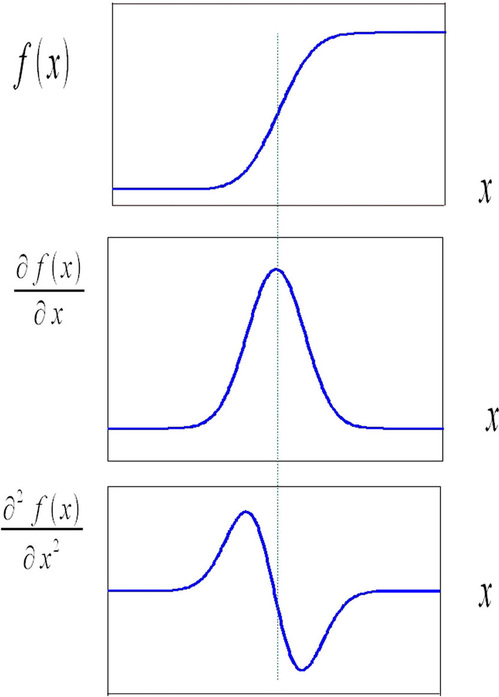
\includegraphics[width=3.7cm]{courbes_gradient.jpg}
	               \end{center}
            	\end{exampleblock}
            \end{frame}
            \begin{frame}
                Script en général et Script-Fu :
                \begin{itemize}
                    \item Objectif: automatiser l'application de plusieurs modifications sur une ou plusieurs images.
                    \item Langages supportés: Scheme, Python, Perl, C\# ...
                    \item Aide: GIMP propose un navigateur de procédures.
                \end{itemize}
            \end{frame}
            \begin{frame}
                Exemple d'un script-fu (Script réalisé en Scheme) :
                \tiny\lstinputlisting{mon-effet.scm}
            \end{frame}
        \subsection{Bénéfices de ce type de développement}
            \begin{frame}{Bénéfices de ce type de développement}
                \tableofcontents[sectionstyle=show/hide,subsectionstyle=show/shaded/hide]
            \end{frame}
            \begin{frame}
                Grace à l'effort des développeurs et à l'intégration continue de scripts et de greffons, le projet a pu s'enrichir au fil des mises à jours.\\
                Exemples d'ajouts lors de l'apparition de la 2.8:
                \begin{itemize}
                    \item Mode une seul fenêtre
                    \item Importation possible de JPEG2000
                    \item Ajout massif de procédures
                \end{itemize}
            \end{frame}
    \section{Conclusion}
        \begin{frame}{Conclusion}
            \tableofcontents[sectionstyle=show/hide,subsectionstyle=show/shaded/hide]
        \end{frame}
        \begin{frame}
            \begin{block}{Conclusion}
            The GIMP est une alternative gratuite vis-à-vis de ses concurrents payants, en matière de traitement d'image (Photoshop, PhotoFiltre, Picasa).\\
            Il est riche en fonctionnalités, puissant et intuitif, son développement est loin d'être terminé.\\
            Il est personnalisable à souhait pour les adeptes de scripting et/ou de programmation C.
            \end{block}
        \end{frame}        
            
\end{document}